\documentclass[xetex,mathserif,serif]{beamer}
\usepackage{polyglossia}
\setdefaultlanguage[babelshorthands=true]{russian}
\usepackage{minted}
\usepackage{tabu}

\useoutertheme{infolines}

\usepackage{fontspec}
\setmainfont{FreeSans}
\newfontfamily{\russianfonttt}{FreeSans}

\definecolor{links}{HTML}{2A1B81}
\hypersetup{colorlinks,linkcolor=,urlcolor=links}

\tabulinesep=0.7mm

\newcommand{\attribution}[1] {
    \vspace{-5mm}\begin{flushright}\begin{scriptsize}\textcolor{gray}{\textcopyright\, #1}\end{scriptsize}\end{flushright}
}

\title{Практика 3: моделирование требований}
\author[Юрий Литвинов]{Юрий Литвинов \newline \textcolor{gray}{\small\texttt{yurii.litvinov@gmail.com}}}

\date{31.01.2022}

\begin{document}
    
    \frame{\titlepage}

    \section{Редакторы}

    \begin{frame}
        \frametitle{Редакторы диаграмм}
        \begin{itemize}
            \item ``Рисовалки''
            \begin{itemize}
                \item Visio
                \item Dia
                \item SmartDraw
                \item LucidChart
                \item \url{http://plantuml.com/}
            \end{itemize}
            \item Полноценные CASE-системы
            \begin{itemize}
                \item Enterprise Architect
                \item Rational Software Architect
                \item MagicDraw
                \item Visual Paradigm
                \item GenMyModel
            \end{itemize}
            \item Инструменты для документирования
            \begin{itemize}
                \item \url{https://www.websequencediagrams.com/}
                \item \url{http://yuml.me/}
                \item \url{https://mermaid-js.github.io/}
            \end{itemize}
        \end{itemize}
    \end{frame}


    \section{Моделирование характеристик}

    \begin{frame}
        \frametitle{Диаграмма характеристик}
        \framesubtitle{Feature Diagram}
        \begin{itemize}
            \item Представляет функциональность системы в виде дерева
            \item Используется в основном для моделирования семейств программных продуктов (Product lines)
        \end{itemize}
        \begin{center}
            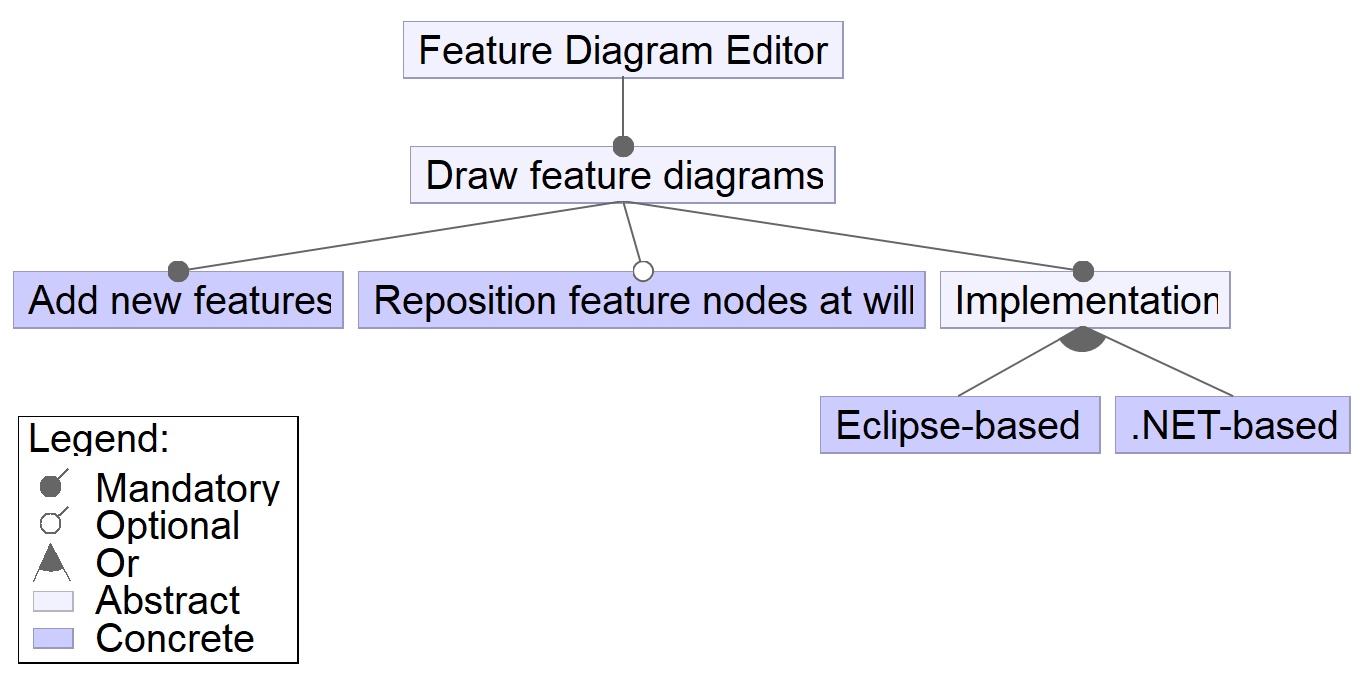
\includegraphics[width=0.6\textwidth]{featureDiagram.png}
        \end{center}
    \end{frame}

    \begin{frame}
        \frametitle{Диаграмма характеристик, пример}
        \begin{center}
            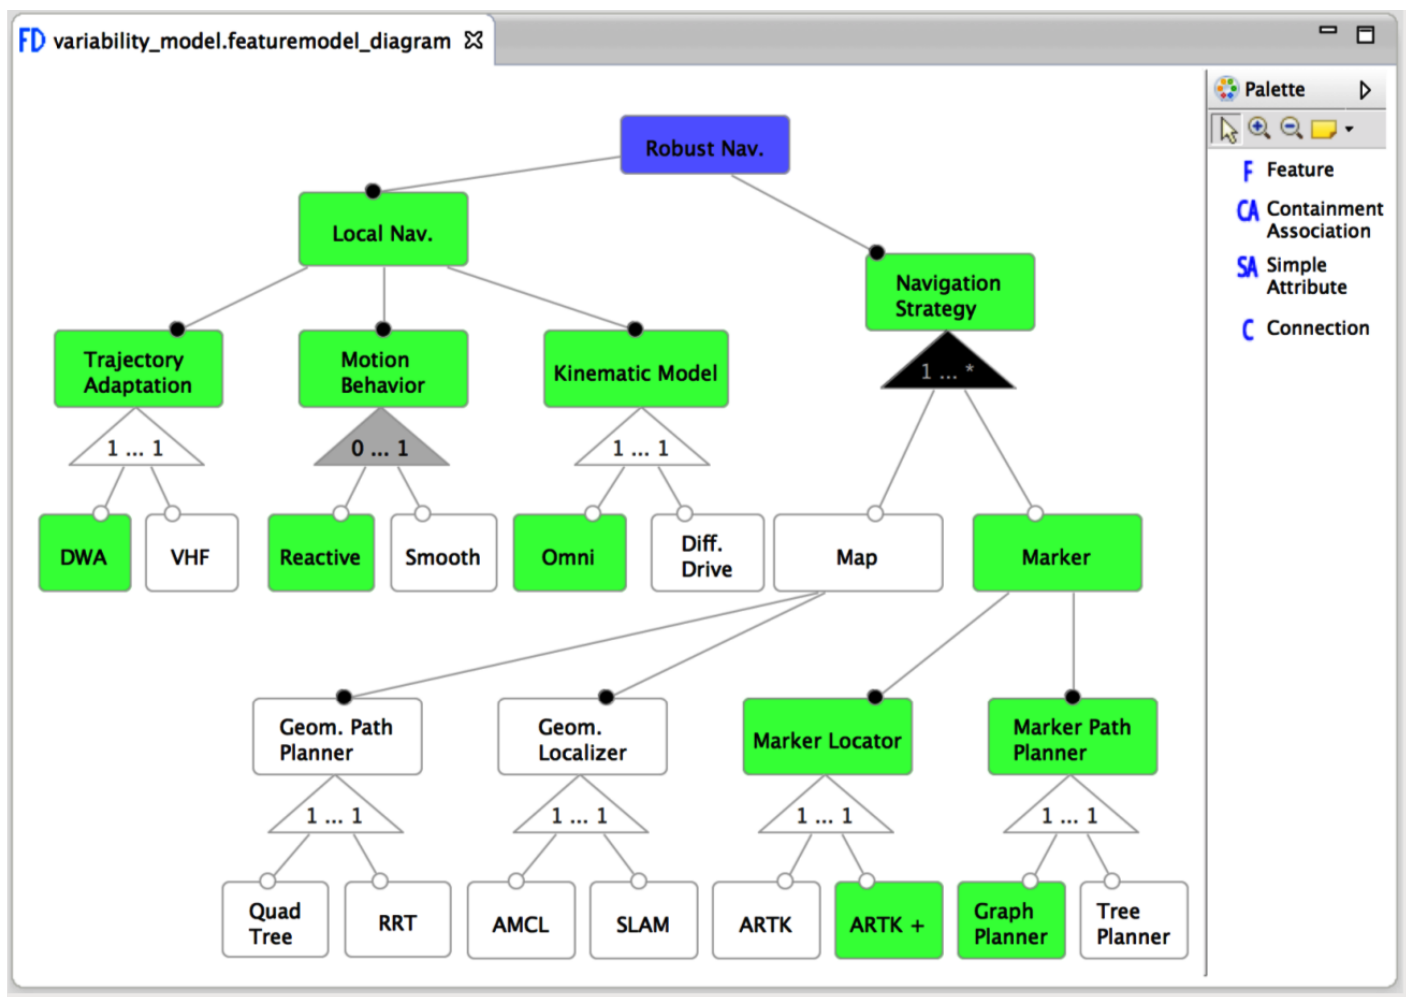
\includegraphics[width=0.8\textwidth]{featureDiagramExample.png}
            \attribution{D. Brugali}
        \end{center}
    \end{frame}

    \begin{frame}
        \frametitle{Feature Tree}
        \begin{center}
            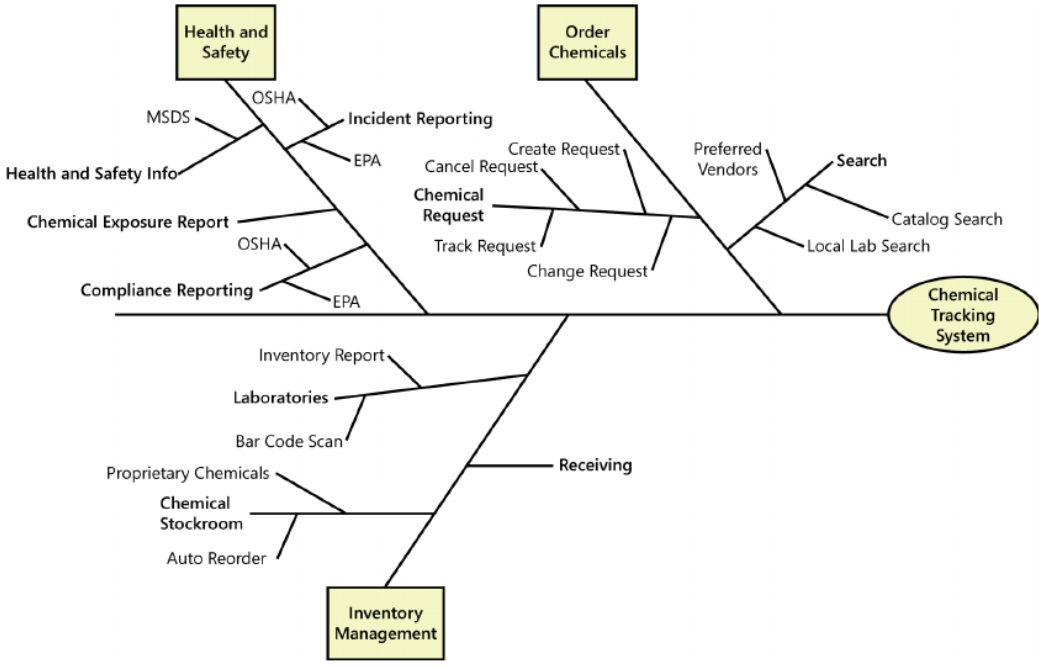
\includegraphics[width=0.8\textwidth]{featureTree.png}
        \end{center}
    \end{frame}

    \section{Моделирование требований в SysML}

    \begin{frame}
        \frametitle{Диаграмма требований, SysML}
        \begin{itemize}
            \item Более формальная нотация дерева фич
        \end{itemize}
        \begin{center}
            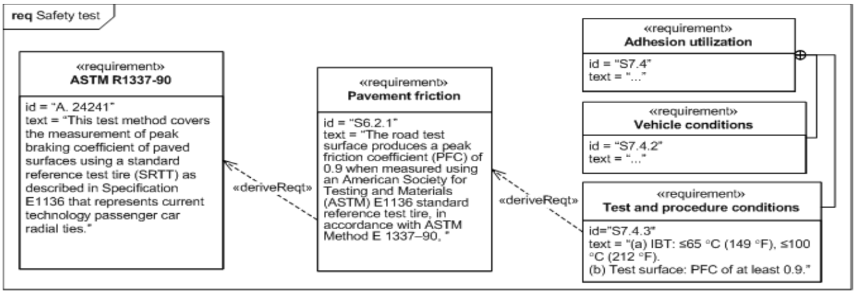
\includegraphics[width=0.6\textwidth]{sysMlRequirementDiagram.png}
            \attribution{OMG SysML 1.4 Specification}
        \end{center}
    \end{frame}

    \begin{frame}
        \frametitle{Диаграмма требований SysML, пример}
        \begin{center}
            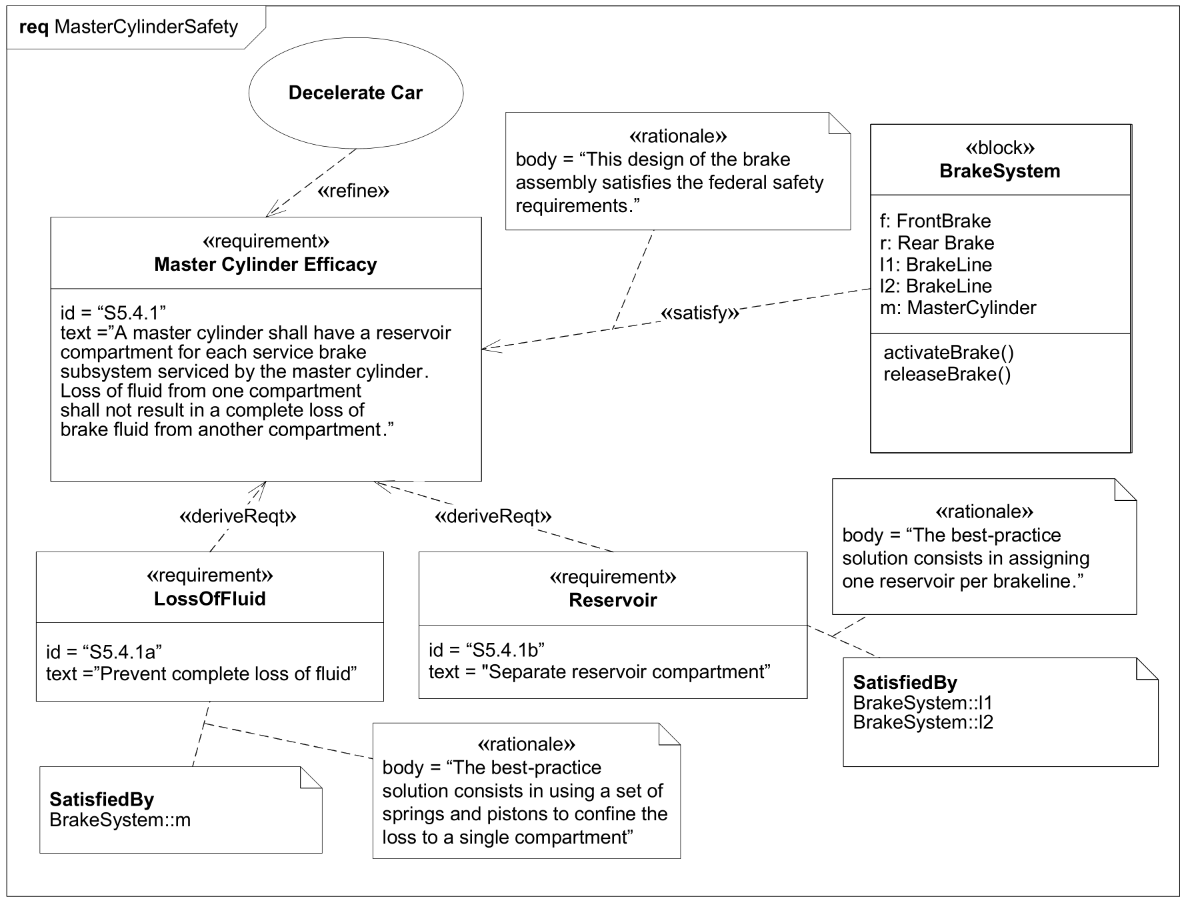
\includegraphics[width=0.75\textwidth]{sysMlRequirementsExample.png}
            \attribution{OMG SysML 1.4 Specification}
        \end{center}
    \end{frame}

    % \begin{frame}
    %     \frametitle{Диаграмма требований SysML и тесты}
    %     \begin{columns}
    %         \begin{column}{0.5\textwidth}
    %             Требования:
    %             \begin{center}
    %                 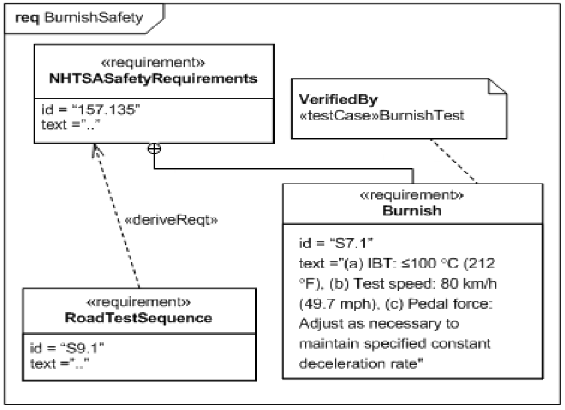
\includegraphics[width=0.8\textwidth]{sysMlRequirementsTest.png}
    %             \end{center}
    %         \end{column}
    %         \begin{column}{0.5\textwidth}
    %             Сценарий тестирования:
    %             \begin{center}
    %                 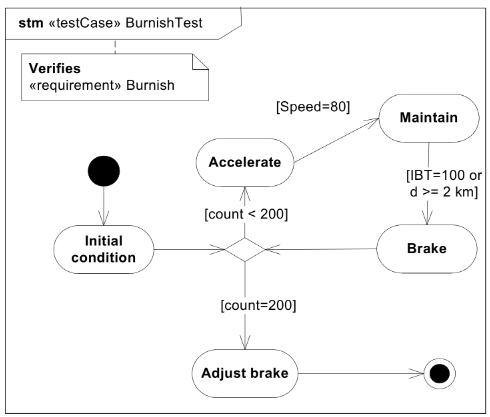
\includegraphics[width=0.9\textwidth]{sysMlRequirementsTestActivity.png}
    %                 \attribution{OMG SysML 1.4 Specification}
    %             \end{center}
    %         \end{column}
    %     \end{columns}
    % \end{frame}

    % \section{Диаграмма активностей UML}

    % \begin{frame}
    %     \frametitle{Диаграмма активностей UML}
    %     \framesubtitle{Диаграммы деятельности}
    %     \begin{columns}
    %         \begin{column}{0.5\textwidth}
    %             \begin{itemize}
    %                 \item Используются для моделирования бизнес-процессов, тоже на первых этапах
    %                 \begin{itemize}
    %                     \item Может быть визуализацией сценария использования
    %                 \end{itemize}
    %                 \item Иногда --- для моделирования алгоритма
    %                 \item Расширенные блок-схемы
    %                 \item Семантика на основе сетей Петри
    %             \end{itemize}
    %         \end{column}
    %         \begin{column}{0.5\textwidth}
    %             \begin{center}
    %                 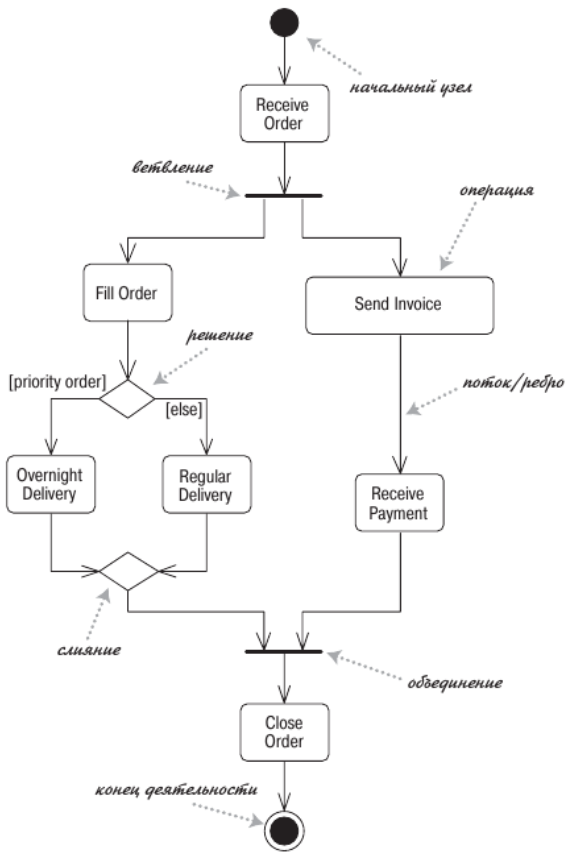
\includegraphics[width=0.7\textwidth]{activityDiagram.png}
    %                 \attribution{М. Фаулер, UML. Основы}
    %             \end{center}
    %         \end{column}
    %     \end{columns}
    % \end{frame}

    % \begin{frame}
    %     \frametitle{Диаграмма активностей, разделы}
    %     \begin{columns}
    %         \begin{column}{0.5\textwidth}
    %             \begin{itemize}
    %                 \item Раздел представляет отдел организации (или организацию), отвечающий за часть работы
    %                 \item Визуализирует поток работ между отделами
    %             \end{itemize}
    %         \end{column}
    %         \begin{column}{0.5\textwidth}
    %             \begin{center}
    %                 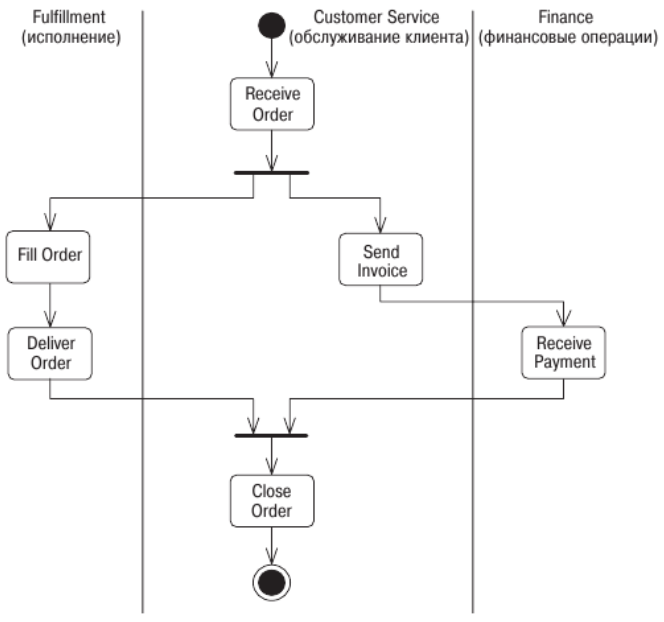
\includegraphics[width=0.9\textwidth]{activitySwimlanes.png}
    %                 \attribution{М. Фаулер, UML. Основы}
    %             \end{center}
    %         \end{column}
    %     \end{columns}
    % \end{frame}

    % \begin{frame}
    %     \frametitle{Диаграмма активностей, сигналы}
    %     \begin{itemize}
    %         \item Для визуализации асинхронных процессов
    %         \item Сигналом может быть посылка документа, запрос и т.д.
    %     \end{itemize}
    %     \begin{center}
    %         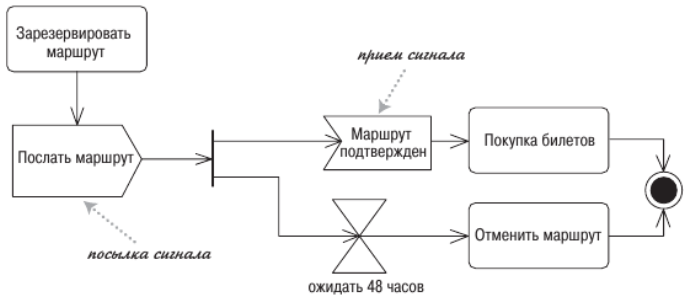
\includegraphics[width=0.6\textwidth]{activitySignals.png}
    %         \attribution{М. Фаулер, UML. Основы}
    %     \end{center}
    % \end{frame}

    \section{BPMN}

    \begin{frame}
        \frametitle{Business Process Model and Notation}
        \begin{itemize}
            \item Версия 1.0 в 2004 году, текущая (2.0.2) --- в 2014
            \item Для описания бизнес-процессов
            \begin{itemize}
                \item Сильно продвинутые диаграммы активностей
                \item Позволяют описывать группы взаимодействующих процессов
                \item Исполнимая семантика
                \item Правила генерации в BPEL
                \begin{itemize}
                    \item Business Process Execution Language
                \end{itemize}
            \end{itemize}
        \end{itemize}
    \end{frame}

    \begin{frame}
        \frametitle{Пример диаграммы}
        \begin{center}
            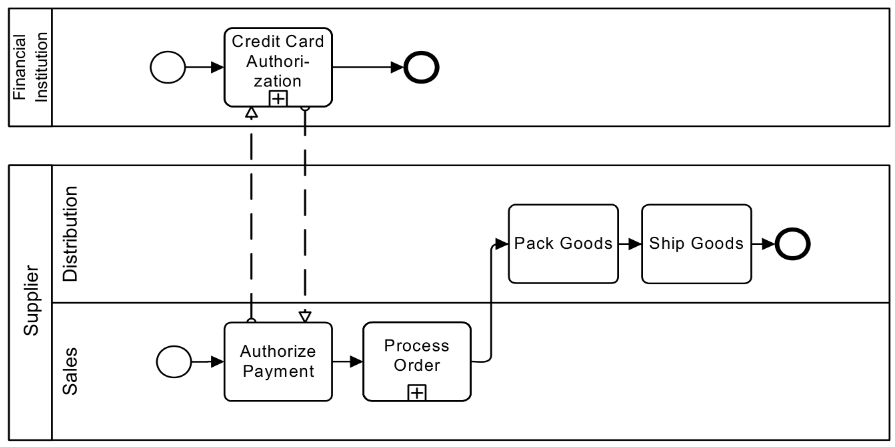
\includegraphics[width=0.9\textwidth]{bpmnExample.png}
            \attribution{OMG BPMN 2.0 Specification}
        \end{center}
    \end{frame}

    \begin{frame}
        \frametitle{События}
        \begin{center}
            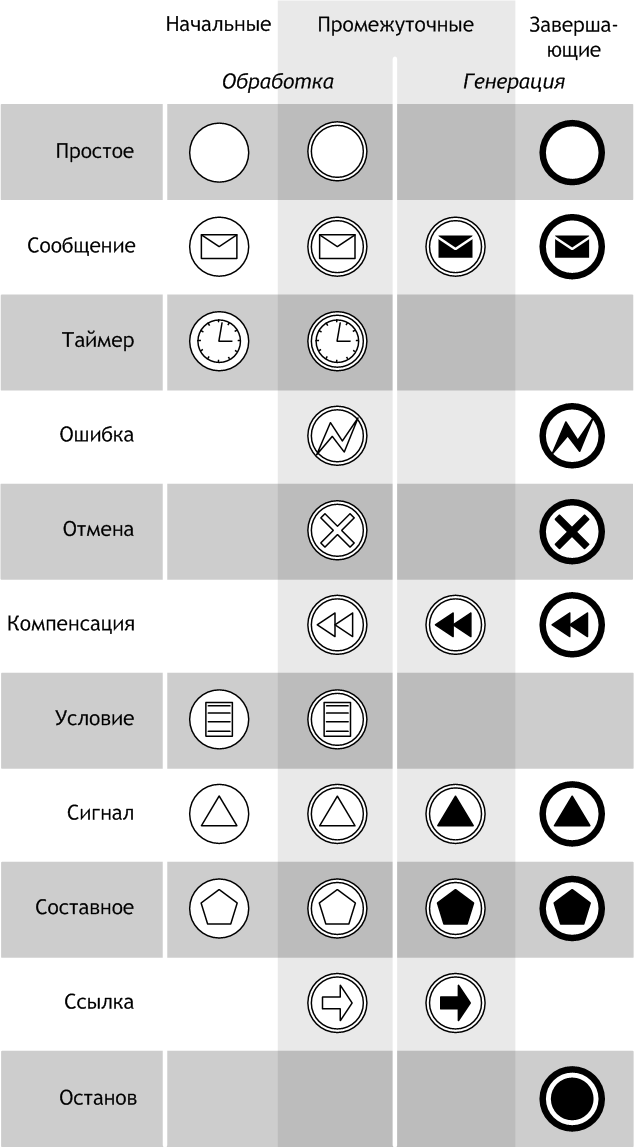
\includegraphics[height=0.8\textheight]{bpmnEvents.png}
            \attribution{\url{https://ru.wikipedia.org/wiki/BPMN}}
        \end{center}
    \end{frame}

    \begin{frame}
        \frametitle{Операторы ветвления}
        \begin{center}
            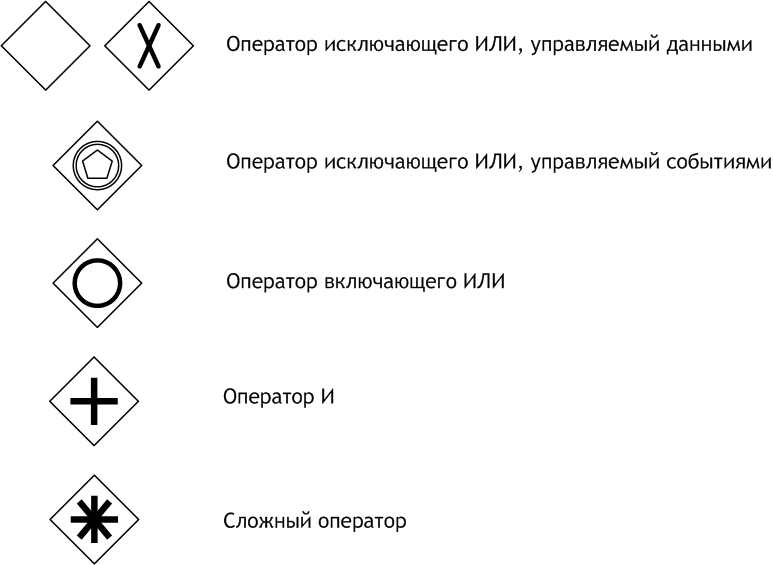
\includegraphics[width=0.5\textwidth]{bpmnGateways.png}
            \attribution{\url{https://ru.wikipedia.org/wiki/BPMN}}
        \end{center}
    \end{frame}

    \begin{frame}
        \frametitle{Диаграмма хореографии}
        \begin{center}
            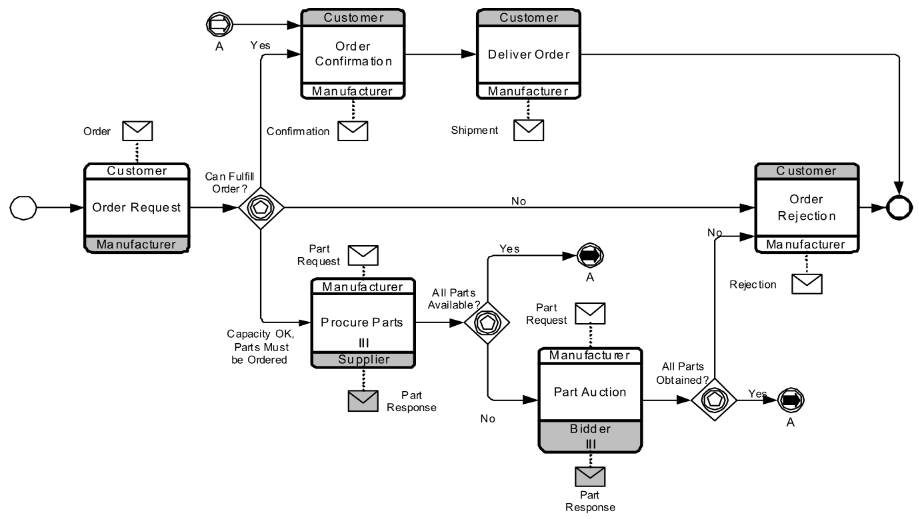
\includegraphics[width=0.9\textwidth]{bpmnChoreography.png}
            \attribution{OMG BPMN 2.0 Specification}
        \end{center}
    \end{frame}

    \begin{frame}
        \frametitle{Диаграмма диалогов}
        \begin{center}
            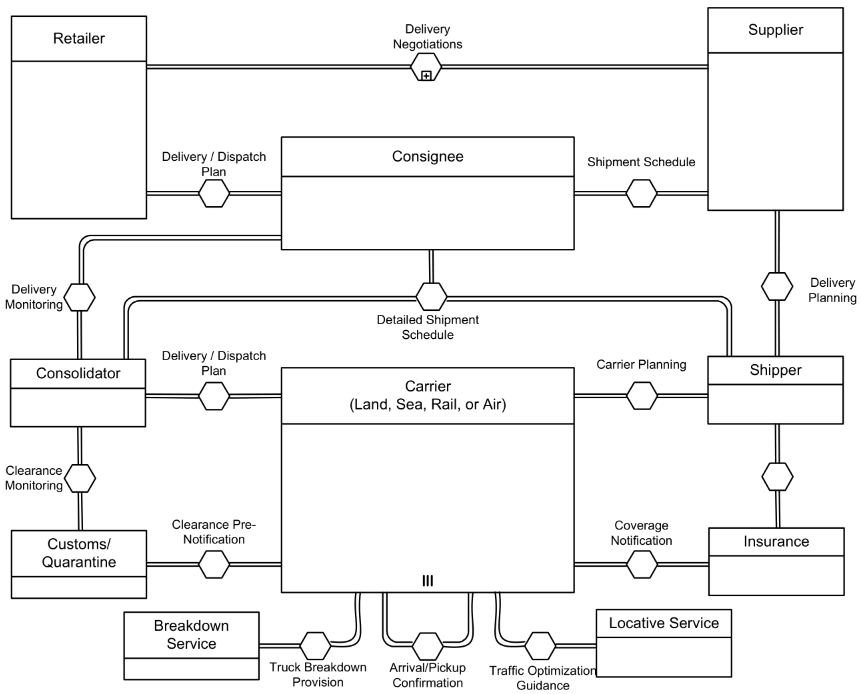
\includegraphics[width=0.7\textwidth]{bpmnConversation.png}
            \attribution{OMG BPMN 2.0 Specification}
        \end{center}
    \end{frame}

    \section{Задачи на практику}

    \begin{frame}
        \frametitle{Задачи на практику}
        В командах по два человека проанализировать запрос \url{https://bit.ly/defects-rfp}, построить по нему:
        \begin{enumerate}
            \item диаграмму случаев использования, описывающую пользователей и случаи использования разрабатываемого приложения
            \item диаграмму активностей для основного бизнес-процесса, поддерживаемого приложением --- регистрации и ремонта дефекта
            \item BPMN-диаграмму для всего бизнес-процесса завода, включая внешних его участников
        \end{enumerate}
        Сдавать в свои репозитории отдельным пуллреквестом. Не забудьте указать, с кем вы в команде.
    \end{frame}

\end{document}
